\documentclass[11pt,a4paper]{scrartcl}
\typearea{12}
\usepackage{graphicx}
\usepackage{pstricks}
\usepackage{listings}
\lstset{language=python}
\pagestyle{headings}
\markright{Computation Neuroscience - 7 vision}

\usepackage{tikz}
%\usepackage{tikzscale}
\usepackage{pgfplots}
\usepackage{color}
\usepackage{pgf}
\usepackage[utf8]{inputenc}
\usetikzlibrary{arrows,automata}
\usetikzlibrary{positioning}


\begin{document}

\section*{Vision}

\subsection*{Introduction} 
This lecture is about vision, they discuss how simple cells in V1 are
modelled and how their behavior may be explained by sparseness.

\subsection*{The visual pathway}
The visual system starts at the eye, where photons are detected and
some denoising occurs; the optical nerve then carries the information
to the thalamus, in the very center of the brain, there it is further
processed and denoised before being relayed on to the visual cortex,
at the very back of the cortex. It is processed in stages in the
cortex with the information being passed forward, as objects are
recognized the information fans out and is integrated with other
signals, from memory, from other sensory modalities and other aspect
of our cognition. The basic pathway is shown in an very old drawing in
Fig.~\ref{fig:Fabrica} and is summarized in
Fig.~\ref{fig:pathway}. One notable aspect is that different sides of
the brain deal with different sides of the visual field, so signal
from the left sides of the retina of both eyes go to the right side of
the brain and signals from the right sides so to the left side.

\begin{figure}
\begin{center}
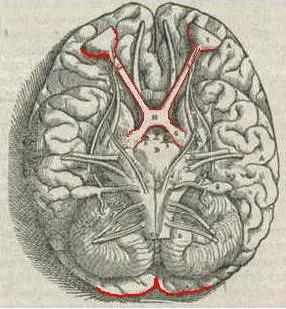
\includegraphics[width=7cm]{Fabrica_VisualSystem.jpg}
\end{center}
\caption{The visual pathway. This is an old drawing due to the C16
  Belgian anatomist Andreas Vesalius taken from his influential 1543
  textbook \textsl{De Humani Corporis Fabrica}. In red are marked the
  retina, the optic nerves, the thalamus where they cross and the
  primary visual cortex. [Image from Wikipedia].\label{fig:Fabrica}}
\end{figure}

Light is detected at the retina, the retina is a surprising organ in
that it is backwards compared to how you'd expect it to be organized;
the layer with light detectors is at the back instead of the
front. Leaving that aside though, basically light is detected in
specialized cells called \textsl{photoreceptors}, these don't spike,
but they do convert light into electrical activity. There are two
types of photoreceptors, the rods, which are important for vision in
low light, and the cones, which are responsible for color vision and
important for vision in normal lighting conditions. The electrically
activity of the photorecptors is passed forward though \textsl{bipolar
  cells} to \textsl{ganglion cells}.

Ganglion cells aggregate activity from a number of photoreptors, along
with activity from some inhibitory cells in the intermediate layer and
their axons form the optic nerve, carrying information to the
thalamus. A sketch of the retina is given in Fig.~\ref{fig:retina}.

\begin{figure}
\begin{center}
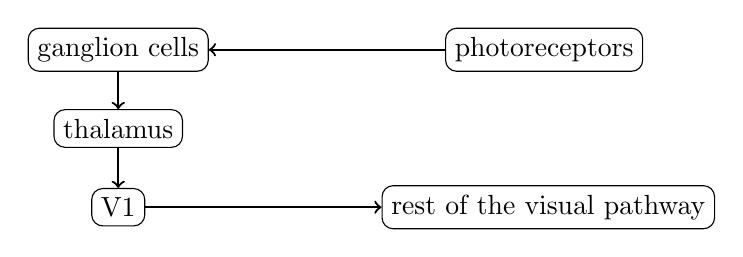
\begin{tikzpicture}
\node[rectangle,rounded corners,draw=black](ph){photoreceptors};
\node[rectangle,rounded corners,draw=black,left = 3cm of ph](g){ganglion cells};
\node[rectangle,rounded corners,draw=black,below of= g](th){thalamus};
\node[rectangle,rounded corners,draw=black,below of= th](v1){V1};
\node[rectangle,rounded corners,draw=black,right = 3cm of v1](v){rest of the visual pathway};
\path (ph) edge[->,thick] (g);
\path (g) edge[->,thick] (th);
\path (th) edge[->,thick] (v1);
\path (v1) edge[->,thick] (v);
\end{tikzpicture}
\end{center}
\caption{The visual pathway. This is a very rough diagram showing the visual pathway; V1 is the first visual area in the cortex.\label{fig:pathway}}
\end{figure}

\begin{figure}
 \begin{center}
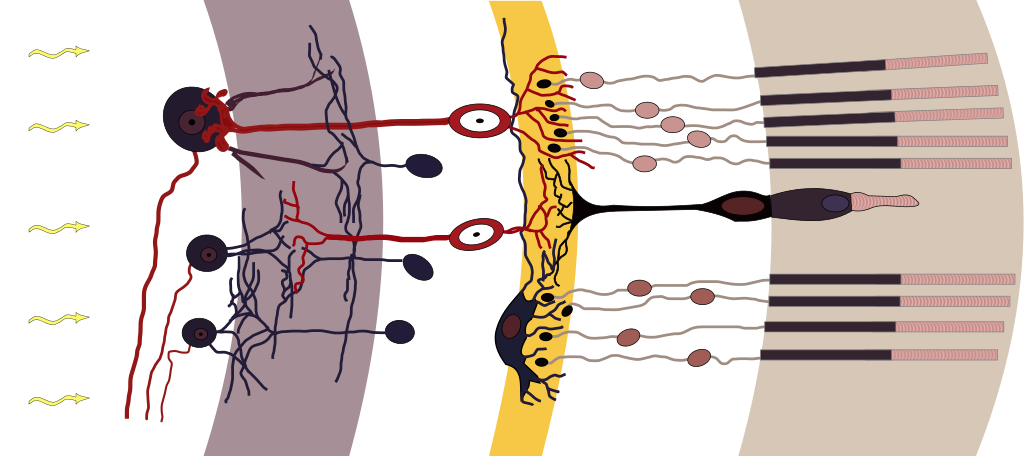
\includegraphics[width=12cm]{retina.png}
\end{center}
\caption{Rods, cones and nerve layers in the retina. The front of the
  eye is on the left. Light (from the left) passes through several
  transparent nerve layers to reach the rods and cones (far right). A
  chemical change in the rods and cones send a signal back to the
  nerves. The signal goes first to the bipolar and horizontal cells
  (yellow layer), then to the amacrine cells and ganglion cells
  (purple layer), then to the optic nerve fibres. The signals are
  processed in these layers. First, the signals start as raw outputs
  of points in the rod and cone cells. Then the nerve layers identify
  simple shapes, such as bright points surrounded by dark points,
  edges, and movement. (Based on a drawing by Ramón y Cajal, 1911.)
  [Caption and drawing taken from Wikipedia: Cajal derivative work:
    Anka Friedrich via Wikimedia Commons]\label{fig:retina}}
\end{figure}

\subsection*{Receptive fields}
\textsl{Receptive fields} are often described as the stimuli giving
the largest response from a neuron. For ganglion and thalamic cells
these are contrast patches, see Fig.~\ref{fig:rf_ganglion}, in
\textsl{on-cells} small patches of the visual field where an
illuminated region surrounded by an unilluminated one causes firing,
different cells will respond to different locations. The width of the
receptive fields vary from the size of full stop at reading distance
in the center, to the size of a page near the periphery. In
\textsl{off-cells} the contrast is reverse, the cell responds to an
unilluminated region surrounded by an illuminated region. In practice
these patterns are the result of excitatory and inhibitory synapses
relaying information from these regions of the visual field.
\begin{center}
\begin{tikzpicture}
\node[](r1){};
\node[right of = r1](r2){};
\node[right of = r2](r3){};
\node[right of = r3](r4){};
\node[right of = r4](r5){};
\node[right of = r5](r6){};
\node[right of = r6](r7){};
\node[right of = r7](r8){};
\node[right of = r8](r9){};
\node[below of = r1](b1){};
\node[right of = b1](b2){};
\node[right of = b2](b3){};
\node[right of = b3](b4){};
\node[right of = b4](b5){};
\node[right of = b5](b6){};
\node[right of = b6](b7){};
\node[right of = b7](b8){};
\node[right of = b8](b9){};
\node[above right = -1mm of b1](bb1){ -};
\node[above right = -1mm of b2](bb2){ -};
\node[above right = -1mm of b3](bb3){ -};
\node[above right = -1mm of b4](bb4){ +};
\node[above right = -1mm of b5](bb5){ +};
\node[above right = -1mm of b6](bb6){ +};
\node[above right = -1mm of b7](bb7){ -};
\node[above right = -1mm of b8](bb8){ -};
\node[above right = -1mm of b9](bb9){ -};
\draw (r1) edge[-o] (b1);
\draw (r2) edge[-o] (b2);
\draw (r3) edge[-o] (b3);
\draw (r4) edge[-<] (b4);
\draw (r5) edge[-<] (b5);
\draw (r6) edge[-<] (b6);
\draw (r7) edge[-o] (b7);
\draw (r8) edge[-o] (b8);
\draw (r9) edge[-o] (b9);
\node[below = -3mm of b1](c1){};
\node[left of  =c1](c0){};
\node[below = -3mm of b9](c9){};
\node[right of =c9](c10){};
\draw (c0) edge (c10);
\node[below = -4mm of b5](c5){};
\node[below of = c5](d5){ganglion cell};
\draw (c5) edge (d5);

%% \node[circle,draw=black, fill=black](a1){};
%% \node[circle,draw=black, fill=white,right of =a1](b1){};
%% \node[circle,draw=black, fill=white,left of =a1](c1){};
%% \node[circle,draw=black, fill=black,below of=a1](a2){};
%% \node[circle,draw=black, fill=white,right of =a2](b2){};
%% \node[circle,draw=black, fill=white,left of =a2](c2){};
%% \node[circle,draw=black, fill=black,above of =a1](a3){};
%% \node[circle,draw=black, fill=white,right of =a3](b3){};
%% \node[circle,draw=black, fill=white,left of =a3](c3){};
%% \node[circle,draw=black,right =3cm of b2](fl){};
%% \node[circle,draw=black,right =3cm of b1](fi){};
%% \node[circle,draw=black,right =3cm of b3,fill=black](fu){};
%% \node[right of=fl](flee){flee};
%% \node[right of=fi](fight){fight};
%% \node[right of=fu](mate){mate};
%% \draw (a1) edge[-o] (fl);
%% \draw (b1) edge[-o] (fl);
%% \draw (c1) edge[-o] (fl);
%% \draw (a2) edge[-o] (fl);
%% \draw (b2) edge[-o] (fl);
%% \draw (c2) edge[-o] (fl);
%% \draw (a3) edge[-o] (fl);
%% \draw (b3) edge[-o] (fl);
%% \draw (c3) edge[-o] (fl);
%% \draw (a1) edge[-o] (fi);
%% \draw (b1) edge[-o] (fi);
%% \draw (c1) edge[-o] (fi);
%% \draw (a2) edge[-o] (fi);
%% \draw (b2) edge[-o] (fi);
%% \draw (c2) edge[-o] (fi);
%% \draw (a3) edge[-o] (fi);
%% \draw (b3) edge[-o] (fi);
%% \draw (c3) edge[-o] (fi);
%% \draw (a1) edge[-o] (fu);
%% \draw (b1) edge[-o] (fu);
%% \draw (c1) edge[-o] (fu);
%% \draw (a2) edge[-o] (fu);
%% \draw (b2) edge[-o] (fu);
%% \draw (c2) edge[-o] (fu);
%% \draw (a3) edge[-o] (fu);
%% \draw (b3) edge[-o] (fu);
%% \draw (c3) edge[-o] (fu);
\end{tikzpicture}
\end{center}
In V1 there
are cells called \textsl{simple cells} and cells called
\textsl{complex cells}; we will concentrate on the simple cells, these
have edge-like receptive fields; different cells respond to particular
orientations in particular locations in the visual field. 

The edge-like receptive fields in V1 were first discovered by Hubel
and Wiesel \cite{HubelWiesel1962a}. The used an electrode to record
from V1 neurons in anaesthetised cat; the moved an edge-like stimulus
around until they found the position that caused the highest firing
rate, they observed that the firing rate depended on orientation as
well as position, see Fig.~\ref{fig:hw} and Fig.~\ref{fig:hw_rf}.

\begin{figure}
\begin{center}

\begin{tikzpicture}
\node[rectangle,text width=3cm,text height=3cm,fill=gray](out1){};
\node[circle,text width=2cm,fill=black](surr1){};
\node[circle,text width=1cm,fill=white](cent1){};
\node[rectangle,text width=3cm,text height=3cm,fill=gray,right = 1cm of out1](out2){};
\node[circle,text width=2cm,fill=white,right = 2cm of surr1](surr2){};
\node[circle,text width=1cm,fill=black,right = 3cm of cent1](cent2){};
\end{tikzpicture}
\end{center}
\caption{On and off cells respond to small contrast patches. \label{fig:rf_ganglion}}
\end{figure}

\begin{figure}
\begin{center}

\begin{tikzpicture}
\node[rectangle,text width=3cm,text height=3cm,fill=gray](out1){};
\draw(0.25,0)[rotate=35,fill=black,draw=gray] ellipse (0.25cm and 0.85cm);
\draw(-0.25,0)[rotate=35,fill=white,draw=gray] ellipse (0.25cm and 0.85cm);

\node[rectangle,text width=3cm,text height=3cm,fill=gray,right = 1cm of out1](out2){};
\draw(4.75,0)[rotate around = {35:(4.25,0)},fill=white,draw=gray] ellipse (0.25cm and 0.85cm);
\draw(3.75,0)[rotate around = {35:(4.25,0)},fill=white,draw=gray] ellipse (0.25cm and 0.85cm);
\draw(4.25,0)[rotate around = {35:(4.25,0)},fill=black,draw=gray] ellipse (0.25cm and 0.85cm);
\end{tikzpicture}
\end{center}
\caption{Simple cells in V1 respond to edges.\label{fig:rf_v1}}
\end{figure}

\begin{figure}
\begin{center}
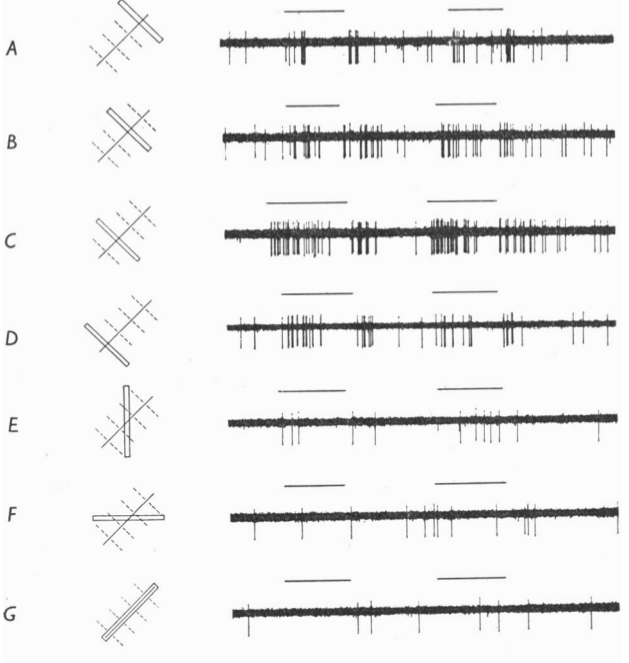
\includegraphics[width=12cm]{HW.png}
\end{center}
\caption{Experimental results from Hubel and Wiesel; the stimulus is a slit that allows light through from a souce, it is $0.125^\circ\times 2.5^\circ$ and is presented during the one-second period marked by the two bars over the plots. In the plots the vertical lines correspond to spikes. [Image from \cite{HubelWiesel1962a}].\label{fig:hw}}
\end{figure}


\begin{figure}
\begin{center}
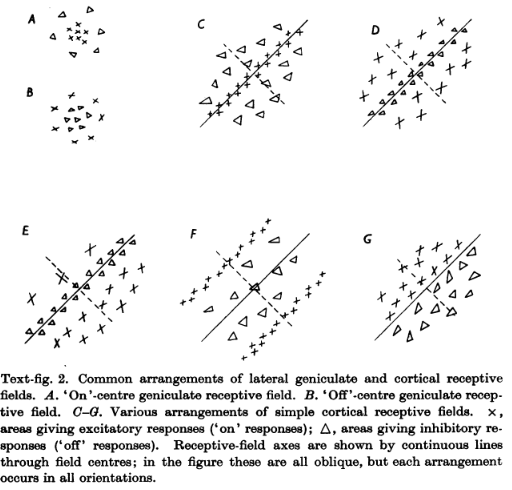
\includegraphics[width=12cm]{HW_rf.png}
\end{center}
\caption{More experimental results from Hubel and Wiesel; here they have mapped out the excitatory (crosses) and inhibitory (triangles) areas for a number of neurons. [Image from \cite{HubelWiesel1962a}].\label{fig:hw_rf}}
\end{figure}


\subsection*{Linear models}


One way to think about it is to imagine the entries in the receptive
field are synapse strengths for inputs from cells responding to
illumination at points in the visual field. To formalize this consider
linear models of the neuron's activity. Let $I_{ij}$ denote the
illumination level at point $(i,j)$ in the visual field, $i$ and $j$
are discrete coordinates, for simplicity we will treat everything
discretely. Now, imagine a linear model of the activity of the neuron,
with the firing rate depending linearly on the illuminations; leaving
out any messing with the firing rate having to be positive, this means
\begin{equation}
\tilde{r}=r_0+\sum w_{ij}I_{ij}
\end{equation}
where $r_0$ is the background firing rate and $w_{ij}$ give the
receptive field. Of course the firing rate of a neuron doesn't satisfy
a linear model but the idea is to choose the linear model which best
approximates the neuron, that is, for example, to choose $w_{ij}$ to
minimize the average square error $\langle (r-\tilde{r})^2\rangle$
between $r$, the observed firing rate and $\tilde{r}$ is the estimated
firing rate from the linear model.

As an example consider
\begin{equation}
[w_{ij}]=\left(\begin{array}{ccccc}
0&0&0&0&0\cr
0&-1/8&-1/8&-1/8&0\cr
0&-1/8&1&-1/8&0\cr
0&-1/8&-1/8&-1/8&0\cr
0&0&0&0&0\end{array}
\right)
\end{equation}
and
\begin{equation}
[I_{ij}]=\left(\begin{array}{ccccc}
1&1&0&0&0\cr
1&1&0&0&0\cr
1&1&0&0&0\cr
1&1&0&0&0\cr
1&1&0&0&0\end{array}
\right)
\end{equation}
which is like a ganglion cell responding to an edge and is illustated
in Fig.~\ref{fig:stim}. If $r_0=2$ say then $\tilde{r}=13/8$.

\begin{figure}
\begin{center}
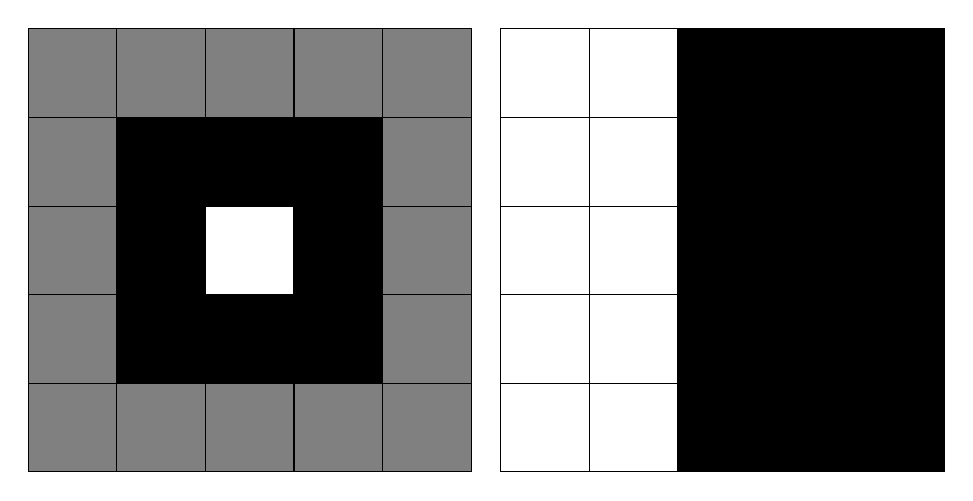
\begin{tikzpicture}
\node at (0,0)[rectangle,text width=0.9cm,text height=0.9cm,draw=black,fill=gray,align=center](00){};
\node at (0,1.125)[rectangle,text width=0.9cm,text height=0.9cm,draw=black,fill=gray,align=center](01){};
\node at (0,2.25)[rectangle,text width=0.9cm,text height=0.9cm,draw=black,fill=gray,align=center](02){};
\node at (0,3.375)[rectangle,text width=0.9cm,text height=0.9cm,draw=black,fill=gray,align=center](04.5){};
\node at(0,4.5)[rectangle,text width=0.9cm,text height=0.9cm,draw=black,fill=gray,align=center](04){};
\node at (1.125,0)[rectangle,text width=0.9cm,text height=0.9cm,draw=black,fill=gray,align=center](10){};
\node at (1.125,1.125)[rectangle,text width=0.9cm,text height=0.9cm,draw=black,fill=black,align=center](11){};
\node at (1.125,2.25)[rectangle,text width=0.9cm,text height=0.9cm,draw=black,fill=black,align=center](12){};
\node at (1.125,3.375)[rectangle,text width=0.9cm,text height=0.9cm,draw=black,fill=black,align=center](14.5){};
\node at(1.125,4.5)[rectangle,text width=0.9cm,text height=0.9cm,draw=black,fill=gray,align=center](14){};
\node at (2.25,0)[rectangle,text width=0.9cm,text height=0.9cm,draw=black,fill=gray,align=center](20){};
\node at (2.25,1.125)[rectangle,text width=0.9cm,text height=0.9cm,draw=black,fill=black,align=center](21){};
\node at (2.25,2.25)[rectangle,text width=0.9cm,text height=0.9cm,draw=black,fill=white,align=center](22){};
\node at (2.25,3.375)[rectangle,text width=0.9cm,text height=0.9cm,draw=black,fill=black,align=center](24.5){};
\node at(2.25,4.5)[rectangle,text width=0.9cm,text height=0.9cm,draw=black,fill=gray,align=center](24){};
\node at (3.375,0)[rectangle,text width=0.9cm,text height=0.9cm,draw=black,fill=gray,align=center](4.50){};
\node at (3.375,1.125)[rectangle,text width=0.9cm,text height=0.9cm,draw=black,fill=black,align=center](4.51){};
\node at (3.375,2.25)[rectangle,text width=0.9cm,text height=0.9cm,draw=black,fill=black,align=center](4.52){};
\node at (3.375,3.375)[rectangle,text width=0.9cm,text height=0.9cm,draw=black,fill=black,align=center](4.54.5){};
\node at(3.375,4.5)[rectangle,text width=0.9cm,text height=0.9cm,draw=black,fill=gray,align=center](4.54){};
\node at (4.5,0)[rectangle,text width=0.9cm,text height=0.9cm,draw=black,fill=gray,align=center](40){};
\node at (4.5,1.125)[rectangle,text width=0.9cm,text height=0.9cm,draw=black,fill=gray,align=center](41){};
\node at (4.5,2.25)[rectangle,text width=0.9cm,text height=0.9cm,draw=black,fill=gray,align=center](42){};
\node at (4.5,3.375)[rectangle,text width=0.9cm,text height=0.9cm,draw=black,fill=gray,align=center](44.5){};
\node at(4.5,4.5)[rectangle,text width=0.9cm,text height=0.9cm,draw=black,fill=gray,align=center](44){};
\node at (6,0)[rectangle,text width=0.9cm,text height=0.9cm,draw=black,fill=white,align=center](00){};
\node at (6,1.125)[rectangle,text width=0.9cm,text height=0.9cm,draw=black,fill=white,align=center](01){};
\node at (6,2.25)[rectangle,text width=0.9cm,text height=0.9cm,draw=black,fill=white,align=center](02){};
\node at (6,3.375)[rectangle,text width=0.9cm,text height=0.9cm,draw=black,fill=white,align=center](04.5){};
\node at(6,4.5)[rectangle,text width=0.9cm,text height=0.9cm,draw=black,fill=white,align=center](04){};
\node at (7.125,0)[rectangle,text width=0.9cm,text height=0.9cm,draw=black,fill=white,align=center](10){};
\node at (7.125,1.125)[rectangle,text width=0.9cm,text height=0.9cm,draw=black,fill=white,align=center](11){};
\node at (7.125,2.25)[rectangle,text width=0.9cm,text height=0.9cm,draw=black,fill=white,align=center](12){};
\node at (7.125,3.375)[rectangle,text width=0.9cm,text height=0.9cm,draw=black,fill=white,align=center](14.5){};
\node at (7.125,4.5)[rectangle,text width=0.9cm,text height=0.9cm,draw=black,fill=white,align=center](14){};
\node at (8.25,0)[rectangle,text width=0.9cm,text height=0.9cm,draw=black,fill=black,align=center](20){};
\node at (8.25,1.125)[rectangle,text width=0.9cm,text height=0.9cm,draw=black,fill=black,align=center](21){};
\node at (8.25,2.25)[rectangle,text width=0.9cm,text height=0.9cm,draw=black,fill=black,align=center](22){};
\node at (8.25,3.375)[rectangle,text width=0.9cm,text height=0.9cm,draw=black,fill=black,align=center](24.5){};
\node at (8.25,4.5)[rectangle,text width=0.9cm,text height=0.9cm,draw=black,fill=black,align=center](24){};
\node at (9.375,0)[rectangle,text width=0.9cm,text height=0.9cm,draw=black,fill=black,align=center](4.50){};
\node at (9.375,1.125)[rectangle,text width=0.9cm,text height=0.9cm,draw=black,fill=black,align=center](4.51){};
\node at (9.375,2.25)[rectangle,text width=0.9cm,text height=0.9cm,draw=black,fill=black,align=center](4.52){};
\node at (9.375,3.375)[rectangle,text width=0.9cm,text height=0.9cm,draw=black,fill=black,align=center](4.54.5){};
\node at (9.375,4.5)[rectangle,text width=0.9cm,text height=0.9cm,draw=black,fill=black,align=center](4.54){};
\node at (10.5,0)[rectangle,text width=0.9cm,text height=0.9cm,draw=black,fill=black,align=center](40){};
\node at (10.5,1.125)[rectangle,text width=0.9cm,text height=0.9cm,draw=black,fill=black,align=center](41){};
\node at (10.5,2.25)[rectangle,text width=0.9cm,text height=0.9cm,draw=black,fill=black,align=center](42){};
\node at (10.5,3.375)[rectangle,text width=0.9cm,text height=0.9cm,draw=black,fill=black,align=center](44.5){};
\node at (10.5,4.5)[rectangle,text width=0.9cm,text height=0.9cm,draw=black,fill=black,align=center](44){};
\end{tikzpicture}
\end{center}
\caption{Receptive field and visual stimulus.\label{fig:stim}}
\end{figure}


\subsection*{Features}

Knowing why V1 receptive fields have the particular stucture they do
is likely to tell us something about what it is that the brain does to
information in the sensory pathways. One idea is that it is related to
feature extraction. To motivate this we will consider a ficticious
world of simplified creatures; imagine we are one of these creatures and wish to
decide how to react to other creatures we encounter. As in the real
world, when we encounter a creature we need to decide between what are
sometimes called the three Fs: fighting, fleeing and mating. Now
imagine that the creatures all have a three by three pattern on their
stomachs:
\begin{center}
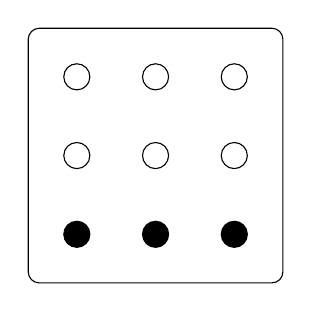
\begin{tikzpicture}
\node[rectangle,rounded corners,draw=black,text width=3cm, text height=3cm](big){};
\node[circle,draw=black, fill=white](a1){};
\node[circle,draw=black, fill=white,right of =a1](b1){};
\node[circle,draw=black, fill=white,left of =a1](c1){};
\node[circle,draw=black, fill=black,below of=a1](a2){};
\node[circle,draw=black, fill=black,right of =a2](b2){};
\node[circle,draw=black, fill=black,left of =a2](c2){};
\node[circle,draw=black, fill=white,above of =a1](a3){};
\node[circle,draw=black, fill=white,right of =a3](b3){};
\node[circle,draw=black, fill=white,left of =a3](c3){};
\end{tikzpicture}
\end{center}
and that creatures to fight have a horizontal strip to the top or the bottom, as above, creatures to flee from, a vertical strip on the left or right, for example
\begin{center}
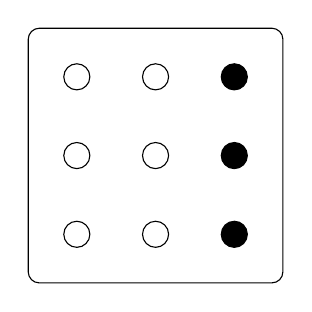
\begin{tikzpicture}
\node[rectangle,rounded corners,draw=black,text width=3cm, text height=3cm](big){};
\node[circle,draw=black, fill=white](a1){};
\node[circle,draw=black, fill=black,right of =a1](b1){};
\node[circle,draw=black, fill=white,left of =a1](c1){};
\node[circle,draw=black, fill=white,below of=a1](a2){};
\node[circle,draw=black, fill=black,right of =a2](b2){};
\node[circle,draw=black, fill=white,left of =a2](c2){};
\node[circle,draw=black, fill=white,above of =a1](a3){};
\node[circle,draw=black, fill=black,right of =a3](b3){};
\node[circle,draw=black, fill=white,left of =a3](c3){};
\end{tikzpicture}
\end{center}
and creatures to mate with, a central line, either horizontal or vertical like:
\begin{center}
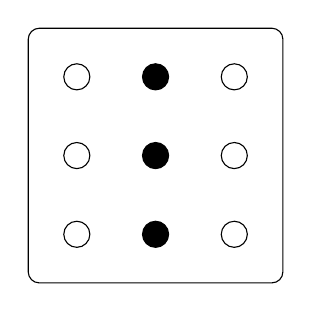
\begin{tikzpicture}
\node[rectangle,rounded corners,draw=black,text width=3cm, text height=3cm](big){};
\node[circle,draw=black, fill=black](a1){};
\node[circle,draw=black, fill=white,right of =a1](b1){};
\node[circle,draw=black, fill=white,left of =a1](c1){};
\node[circle,draw=black, fill=black,below of=a1](a2){};
\node[circle,draw=black, fill=white,right of =a2](b2){};
\node[circle,draw=black, fill=white,left of =a2](c2){};
\node[circle,draw=black, fill=black,above of =a1](a3){};
\node[circle,draw=black, fill=white,right of =a3](b3){};
\node[circle,draw=black, fill=white,left of =a3](c3){};
\end{tikzpicture}
\end{center}

Now, imagine processing this information so as to rapidly decide what
to do, the simplest neural network to process the patterns would look
like
\begin{center}
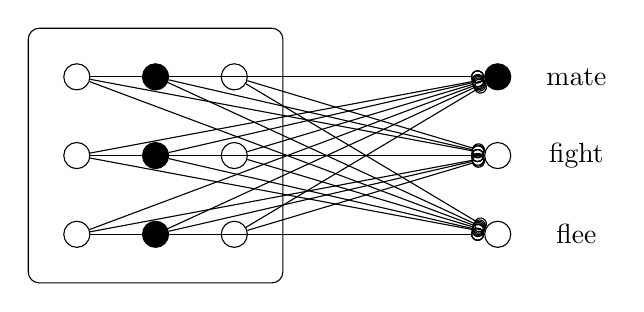
\begin{tikzpicture}
\node[rectangle,rounded corners,draw=black,text width=3cm, text height=3cm](big){};
\node[circle,draw=black, fill=black](a1){};
\node[circle,draw=black, fill=white,right of =a1](b1){};
\node[circle,draw=black, fill=white,left of =a1](c1){};
\node[circle,draw=black, fill=black,below of=a1](a2){};
\node[circle,draw=black, fill=white,right of =a2](b2){};
\node[circle,draw=black, fill=white,left of =a2](c2){};
\node[circle,draw=black, fill=black,above of =a1](a3){};
\node[circle,draw=black, fill=white,right of =a3](b3){};
\node[circle,draw=black, fill=white,left of =a3](c3){};
\node[circle,draw=black,right =3cm of b2](fl){};
\node[circle,draw=black,right =3cm of b1](fi){};
\node[circle,draw=black,right =3cm of b3,fill=black](fu){};
\node[right of=fl](flee){flee};
\node[right of=fi](fight){fight};
\node[right of=fu](mate){mate};
\draw (a1) edge[-o] (fl);
\draw (b1) edge[-o] (fl);
\draw (c1) edge[-o] (fl);
\draw (a2) edge[-o] (fl);
\draw (b2) edge[-o] (fl);
\draw (c2) edge[-o] (fl);
\draw (a3) edge[-o] (fl);
\draw (b3) edge[-o] (fl);
\draw (c3) edge[-o] (fl);
\draw (a1) edge[-o] (fi);
\draw (b1) edge[-o] (fi);
\draw (c1) edge[-o] (fi);
\draw (a2) edge[-o] (fi);
\draw (b2) edge[-o] (fi);
\draw (c2) edge[-o] (fi);
\draw (a3) edge[-o] (fi);
\draw (b3) edge[-o] (fi);
\draw (c3) edge[-o] (fi);
\draw (a1) edge[-o] (fu);
\draw (b1) edge[-o] (fu);
\draw (c1) edge[-o] (fu);
\draw (a2) edge[-o] (fu);
\draw (b2) edge[-o] (fu);
\draw (c2) edge[-o] (fu);
\draw (a3) edge[-o] (fu);
\draw (b3) edge[-o] (fu);
\draw (c3) edge[-o] (fu);
\end{tikzpicture}
\end{center}
Clearly this would be very hard to learn; the connection from, say the
bottom middle node is on in two of the patterns above despite these patterns
corresponding to different types of creature. 

A far better strategy would be to first learn features and then learn
the association between these features and the creature type. Here the features are clearly the horizontal and vertical bars
\begin{center}
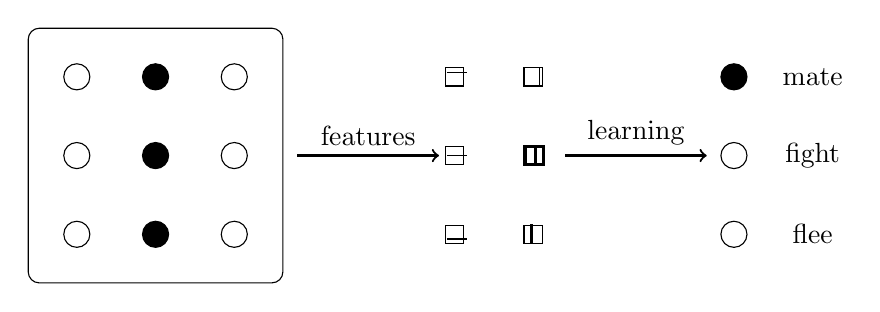
\begin{tikzpicture}
\node[rectangle,rounded corners,draw=black,text width=3cm, text height=3cm](big){};
\node[circle,draw=black, fill=black](a1){};
\node[circle,draw=black, fill=white,right of =a1](b1){};
\node[circle,draw=black, fill=white,left of =a1](c1){};
\node[circle,draw=black, fill=black,below of=a1](a2){};
\node[circle,draw=black, fill=white,right of =a2](b2){};
\node[circle,draw=black, fill=white,left of =a2](c2){};
\node[circle,draw=black, fill=black,above of =a1](a3){};
\node[circle,draw=black, fill=white,right of =a3](b3){};
\node[circle,draw=black, fill=white,left of =a3](c3){};
\node[circle,draw=black,right =6cm of b2](fl){};
\node[circle,draw=black,right =6cm of b1](fi){};
\node[circle,draw=black,right =6cm of b3,fill=black](fu){};
\node[right of=fl](flee){flee};
\node[right of=fi](fight){fight};
\node[right of=fu](mate){mate};
\node[rectangle,draw=black,right=2.5cm of b2](h1){};
\node[rectangle,draw=black,right=2.5cm of b1](h2){};
\node[rectangle,draw=black,right=2.5cm of b3](h3){};
\node[rectangle,draw=black,right=3.5cm of b2](v1){};
\node[rectangle,draw=black,very thick,right=3.5cm of b1](v2){};
\node[rectangle,draw=black,right=3.5cm of b3](v3){};
\draw (3.7,-1.06) -- (3.95,-1.06);
\draw (3.7,1.06) -- (3.95,1.06);
\draw (3.7,0.00) -- (3.95,0.00);
\draw (4.775,-0.875) edge[thick] (4.775,-1.125);
\draw (4.875,0.875) -- (4.875,1.125);
\draw (4.825,-0.125) edge[thick] (4.825,0.125);
\draw (1.8,0) edge[thick,->] node[above]{features} (3.6,0);
\draw (5.2,0) edge[thick,->] node[above]{learning} (7.0,0);
\end{tikzpicture}
\end{center}
In this case the problem has been split in two; first the connections
summarized as \lq{}features\rq{} above are learned from the data,
possibly using the sort of correllation structure learning provided
for by STDP, the interpretation of these feature is then learned, this
is clearly easier, the connections summarized as \lq{}learning\rq{}
have a far simpler task, which is good, since it is crucial to learn
this sort of salient ecological information quickly.


\subsection*{Feature selection}
Here we will consider what properties we would expect features to
have. To do this lets imagine that there are neurons that correspond
to the features and their activity represents the image. Say the
feature neurons each has a receptive field and responds linearly and
for simplicity we will leave out the background firing rate: for the
$s$th feature neuron
\begin{equation}
a_s=\sum_{ij} w^s_{ij}I_{ij}
\end{equation}
and conversely, the output can be represented by
\begin{equation}
I_{ij}=\sum_{s} a^sW^s_{ij}
\end{equation}

\subsubsection*{Confusing aside - rate versus reconstruction}
The slightly confusing thing here is that we are moving between the linear model and the reconstruction. We do this all the time with vectors:
\begin{equation}
\textbf{v}=v_1\textbf{i}+v_2\textbf{j}+v_3\textbf{k}
\end{equation}
is the reconstruction where the corresponding project, for example
\begin{equation}
v_1-\textbf{v}\cdot\textbf{i}
\end{equation}
is like the linear model. However, the situation in this case is more striaght-forward, because the basis vectors are orthonormal
\begin{equation}
\textbf{i}\cdot\textbf{j}=\textbf{j}\cdot\textbf{k}=\textbf{k}\cdot\textbf{i}=0
\end{equation}
and
\begin{equation}
\textbf{i}\cdot\textbf{i}=\textbf{j}\cdot\textbf{j}=\textbf{k}\cdot\textbf{k}=1
\end{equation}
the same basis vector appears in the reconstruction and the
projection: the coeffient $v_1$ of $\textbf{i}$ in the reconstruction
is the projection of $\textbf{v}$ onto $\textbf{i}$. However, in the
case of vision the basis elements, the $W^s_{ij}$ and $w^s_{ij}$ are
not orthonormal and therefore are not the same, working out the
relationship between involves vectorizing the matrix indices $i$ and
$j$, so we won't go into it here, morally one is the inverse transpose
of the other. In fact, here we will consider an example where the
dimensions are different, where the image patches are $3\times 3$ but
there are only six features, so $s=1\ldots 6$. This means that the
reconstructed image may not be equal the original image and will just
be an approximation to it.

As an example, lets have
\begin{center}
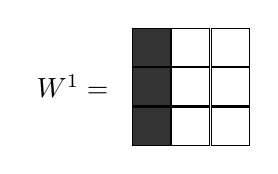
\begin{tikzpicture}
\node at (-1,0.5){$W^1=$};
\node at (0,0)[rectangle,text width=0.25cm,text height=0.25cm,draw=black,fill=black!80,align=center](00){};
\node at (0,0.5)[rectangle,text width=0.25cm,text height=0.25cm,draw=black,fill=black!80,align=center](01){};
\node at (0,1)[rectangle,text width=0.25cm,text height=0.25cm,draw=black,fill=black!80,align=center](02){};
\node at (0.5,0)[rectangle,text width=0.25cm,text height=0.25cm,draw=black,fill=black!0,align=center](10){};
\node at (0.5,0.5)[rectangle,text width=0.25cm,text height=0.25cm,draw=black,fill=black!0,align=center](11){};
\node at (0.5,1)[rectangle,text width=0.25cm,text height=0.25cm,draw=black,fill=black!0,align=center](12){};
\node at (1,0)[rectangle,text width=0.25cm,text height=0.25cm,draw=black,fill=black!0,align=center](20){};
\node at (1,0.5)[rectangle,text width=0.25cm,text height=0.25cm,draw=black,fill=black!0,align=center](21){};
\node at (1,1)[rectangle,text width=0.25cm,text height=0.25cm,draw=black,fill=black!0,align=center](22){};
\end{tikzpicture}
\quad
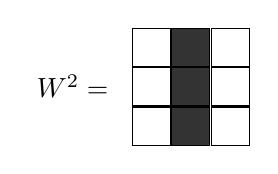
\begin{tikzpicture}
\node at (-1,0.5){$W^2=$};
\node at (0,0)[rectangle,text width=0.25cm,text height=0.25cm,draw=black,fill=black!0,align=center](00){};
\node at (0,0.5)[rectangle,text width=0.25cm,text height=0.25cm,draw=black,fill=black!0,align=center](01){};
\node at (0,1)[rectangle,text width=0.25cm,text height=0.25cm,draw=black,fill=black!0,align=center](02){};
\node at (0.5,0)[rectangle,text width=0.25cm,text height=0.25cm,draw=black,fill=black!80,align=center](10){};
\node at (0.5,0.5)[rectangle,text width=0.25cm,text height=0.25cm,draw=black,fill=black!80,align=center](11){};
\node at (0.5,1)[rectangle,text width=0.25cm,text height=0.25cm,draw=black,fill=black!80,align=center](12){};
\node at (1,0)[rectangle,text width=0.25cm,text height=0.25cm,draw=black,fill=black!0,align=center](20){};
\node at (1,0.5)[rectangle,text width=0.25cm,text height=0.25cm,draw=black,fill=black!0,align=center](21){};
\node at (1,1)[rectangle,text width=0.25cm,text height=0.25cm,draw=black,fill=black!0,align=center](22){};
\end{tikzpicture}
\quad
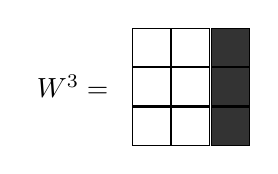
\begin{tikzpicture}
\node at (-1,0.5){$W^3=$};
\node at (0,0)[rectangle,text width=0.25cm,text height=0.25cm,draw=black,fill=black!0,align=center](00){};
\node at (0,0.5)[rectangle,text width=0.25cm,text height=0.25cm,draw=black,fill=black!0,align=center](01){};
\node at (0,1)[rectangle,text width=0.25cm,text height=0.25cm,draw=black,fill=black!0,align=center](02){};
\node at (0.5,0)[rectangle,text width=0.25cm,text height=0.25cm,draw=black,fill=black!0,align=center](10){};
\node at (0.5,0.5)[rectangle,text width=0.25cm,text height=0.25cm,draw=black,fill=black!0,align=center](11){};
\node at (0.5,1)[rectangle,text width=0.25cm,text height=0.25cm,draw=black,fill=black!0,align=center](12){};
\node at (1,0)[rectangle,text width=0.25cm,text height=0.25cm,draw=black,fill=black!80,align=center](20){};
\node at (1,0.5)[rectangle,text width=0.25cm,text height=0.25cm,draw=black,fill=black!80,align=center](21){};
\node at (1,1)[rectangle,text width=0.25cm,text height=0.25cm,draw=black,fill=black!80,align=center](22){};
\end{tikzpicture}
\end{center}
\begin{center}
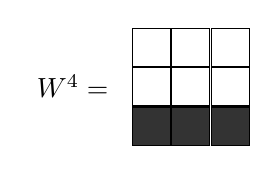
\begin{tikzpicture}
\node at (-1,0.5){$W^4=$};
\node at (0,0)[rectangle,text width=0.25cm,text height=0.25cm,draw=black,fill=black!80,align=center](00){};
\node at (0,0.5)[rectangle,text width=0.25cm,text height=0.25cm,draw=black,fill=black!0,align=center](01){};
\node at (0,1)[rectangle,text width=0.25cm,text height=0.25cm,draw=black,fill=black!0,align=center](02){};
\node at (0.5,0)[rectangle,text width=0.25cm,text height=0.25cm,draw=black,fill=black!80,align=center](10){};
\node at (0.5,0.5)[rectangle,text width=0.25cm,text height=0.25cm,draw=black,fill=black!0,align=center](11){};
\node at (0.5,1)[rectangle,text width=0.25cm,text height=0.25cm,draw=black,fill=black!0,align=center](12){};
\node at (1,0)[rectangle,text width=0.25cm,text height=0.25cm,draw=black,fill=black!80,align=center](20){};
\node at (1,0.5)[rectangle,text width=0.25cm,text height=0.25cm,draw=black,fill=black!0,align=center](21){};
\node at (1,1)[rectangle,text width=0.25cm,text height=0.25cm,draw=black,fill=black!0,align=center](22){};
\end{tikzpicture}
\quad
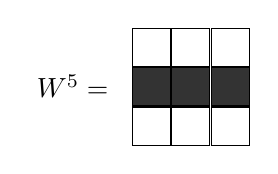
\begin{tikzpicture}
\node at (-1,0.5){$W^5=$};
\node at (0,0)[rectangle,text width=0.25cm,text height=0.25cm,draw=black,fill=black!0,align=center](00){};
\node at (0,0.5)[rectangle,text width=0.25cm,text height=0.25cm,draw=black,fill=black!80,align=center](01){};
\node at (0,1)[rectangle,text width=0.25cm,text height=0.25cm,draw=black,fill=black!0,align=center](02){};
\node at (0.5,0)[rectangle,text width=0.25cm,text height=0.25cm,draw=black,fill=black!0,align=center](10){};
\node at (0.5,0.5)[rectangle,text width=0.25cm,text height=0.25cm,draw=black,fill=black!80,align=center](11){};
\node at (0.5,1)[rectangle,text width=0.25cm,text height=0.25cm,draw=black,fill=black!0,align=center](12){};
\node at (1,0)[rectangle,text width=0.25cm,text height=0.25cm,draw=black,fill=black!0,align=center](20){};
\node at (1,0.5)[rectangle,text width=0.25cm,text height=0.25cm,draw=black,fill=black!80,align=center](21){};
\node at (1,1)[rectangle,text width=0.25cm,text height=0.25cm,draw=black,fill=black!0,align=center](22){};
\end{tikzpicture}
\quad
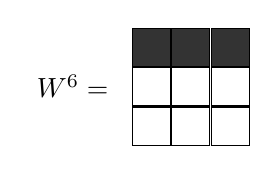
\begin{tikzpicture}
\node at (-1,0.5){$W^6=$};
\node at (0,0)[rectangle,text width=0.25cm,text height=0.25cm,draw=black,fill=black!0,align=center](00){};
\node at (0,0.5)[rectangle,text width=0.25cm,text height=0.25cm,draw=black,fill=black!0,align=center](01){};
\node at (0,1)[rectangle,text width=0.25cm,text height=0.25cm,draw=black,fill=black!80,align=center](02){};
\node at (0.5,0)[rectangle,text width=0.25cm,text height=0.25cm,draw=black,fill=black!0,align=center](10){};
\node at (0.5,0.5)[rectangle,text width=0.25cm,text height=0.25cm,draw=black,fill=black!0,align=center](11){};
\node at (0.5,1)[rectangle,text width=0.25cm,text height=0.25cm,draw=black,fill=black!80,align=center](12){};
\node at (1,0)[rectangle,text width=0.25cm,text height=0.25cm,draw=black,fill=black!0,align=center](20){};
\node at (1,0.5)[rectangle,text width=0.25cm,text height=0.25cm,draw=black,fill=black!0,align=center](21){};
\node at (1,1)[rectangle,text width=0.25cm,text height=0.25cm,draw=black,fill=black!80,align=center](22){};
\end{tikzpicture}
\end{center}
where the almost-black corresponds to one and white to zero, so put another way
\begin{equation}
[W^1_{ij}]=\left(\begin{array}{lll}1&0&0\\1&0&0\\1&0&0\end{array}\right)
\end{equation}
Now consider the example visual input
\begin{center}
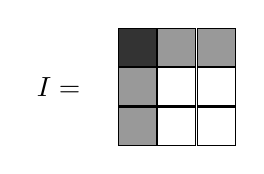
\begin{tikzpicture}
\node at (-1,0.5){$I=$};
\node at (0,0)[rectangle,text width=0.25cm,text height=0.25cm,draw=black,fill=black!40,align=center](00){};
\node at (0,0.5)[rectangle,text width=0.25cm,text height=0.25cm,draw=black,fill=black!40,align=center](01){};
\node at (0,1)[rectangle,text width=0.25cm,text height=0.25cm,draw=black,fill=black!80,align=center](02){};
\node at (0.5,0)[rectangle,text width=0.25cm,text height=0.25cm,draw=black,fill=black!0,align=center](10){};
\node at (0.5,0.5)[rectangle,text width=0.25cm,text height=0.25cm,draw=black,fill=black!0,align=center](11){};
\node at (0.5,1)[rectangle,text width=0.25cm,text height=0.25cm,draw=black,fill=black!40,align=center](12){};
\node at (1,0)[rectangle,text width=0.25cm,text height=0.25cm,draw=black,fill=black!0,align=center](20){};
\node at (1,0.5)[rectangle,text width=0.25cm,text height=0.25cm,draw=black,fill=black!0,align=center](21){};
\node at (1,1)[rectangle,text width=0.25cm,text height=0.25cm,draw=black,fill=black!40,align=center](22){};
\end{tikzpicture}
\end{center}
This would correspond to $a=(0.5,0,0,0,0,0.5)$ or
\begin{center}
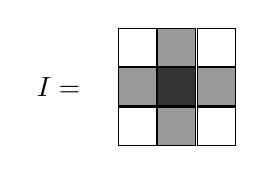
\begin{tikzpicture}
\node at (-1,0.5){$I=$};
\node at (0,0)[rectangle,text width=0.25cm,text height=0.25cm,draw=black,fill=black!0,align=center](00){};
\node at (0,0.5)[rectangle,text width=0.25cm,text height=0.25cm,draw=black,fill=black!40,align=center](01){};
\node at (0,1)[rectangle,text width=0.25cm,text height=0.25cm,draw=black,fill=black!0,align=center](02){};
\node at (0.5,0)[rectangle,text width=0.25cm,text height=0.25cm,draw=black,fill=black!40,align=center](10){};
\node at (0.5,0.5)[rectangle,text width=0.25cm,text height=0.25cm,draw=black,fill=black!80,align=center](11){};
\node at (0.5,1)[rectangle,text width=0.25cm,text height=0.25cm,draw=black,fill=black!40,align=center](12){};
\node at (1,0)[rectangle,text width=0.25cm,text height=0.25cm,draw=black,fill=black!0,align=center](20){};
\node at (1,0.5)[rectangle,text width=0.25cm,text height=0.25cm,draw=black,fill=black!40,align=center](21){};
\node at (1,1)[rectangle,text width=0.25cm,text height=0.25cm,draw=black,fill=black!0,align=center](22){};
\end{tikzpicture}
\end{center}
corresponds to $a=(0,0.5,0,0,0.5,0)$ whereas
\begin{center}
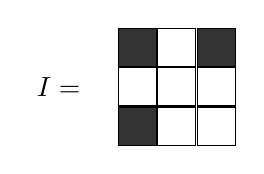
\begin{tikzpicture}
\node at (-1,0.5){$I=$};
\node at (0,0)[rectangle,text width=0.25cm,text height=0.25cm,draw=black,fill=black!80,align=center](00){};
\node at (0,0.5)[rectangle,text width=0.25cm,text height=0.25cm,draw=black,fill=black!0,align=center](01){};
\node at (0,1)[rectangle,text width=0.25cm,text height=0.25cm,draw=black,fill=black!80,align=center](02){};
\node at (0.5,0)[rectangle,text width=0.25cm,text height=0.25cm,draw=black,fill=black!0,align=center](10){};
\node at (0.5,0.5)[rectangle,text width=0.25cm,text height=0.25cm,draw=black,fill=black!0,align=center](11){};
\node at (0.5,1)[rectangle,text width=0.25cm,text height=0.25cm,draw=black,fill=black!0,align=center](12){};
\node at (1,0)[rectangle,text width=0.25cm,text height=0.25cm,draw=black,fill=black!0,align=center](20){};
\node at (1,0.5)[rectangle,text width=0.25cm,text height=0.25cm,draw=black,fill=black!0,align=center](21){};
\node at (1,1)[rectangle,text width=0.25cm,text height=0.25cm,draw=black,fill=black!80,align=center](22){};
\end{tikzpicture}
\end{center}
lies outside the six-dimensional subspace spanned by the features.

\subsubsection*{Sparseness}

The question now is what principle to use to select the features. One
idea, due to \cite{OlshausenField1996a.OlshausenField1997a}, is to use sparseness. Going back to the example
with creatures with patterned bellies, looking at flee-from animal,
for example, three dots are black so among neurons that code for
individual dots three would be active, but among neurons coding for
vertical or horizontal lines, only one would be active. 

Of course this is a very artificial made-up example, the it thought
that \lq{}sparseness\rq{} is a good way to define features
\cite{OlshausenField1996a,OlshausenField1997a}. Very roughly, the
fewer neurons needed to reconstruct an image, the more of the image
each neuron is coding for; for this to work without having a vast
number of neurons covering every possible combination of pixels, the
neurons must code for features, piece of image that occur
regularly. The assumption, in short, is that all the images are mostly
made of the same few building blocks.

The idea is as follows, let $I$ be a image and $\tilde{I}$ an approximation to that image formed using features
\begin{equation}
\tilde{I}_{ij}=\sum_{s}a_sW^s_{ij}
\end{equation}
Now $W^s$ could be under-complete, like above, or over-complete, as it
may be in the visual system, or the dimensions could be chosen to match. Either way, even if the basis is not under-complete, $\tilde{I}$ is an approximation because the $a_s$ are not just chosen to give an accurate reconstruction, but to do so in a sparse way; the are chosen to minimize
\begin{equation}
E=\sum_{ij}(I_{ij}-\tilde{I}_{ij})^2+\beta\sum_s f(a_s)
\end{equation}
This has two terms, the first measures the square error between $I$ and $\tilde{I}$, the second is intended as a measure of sparseness, there are different choices possible, one example would be
\begin{equation}
f(x)=\log_2(1+x^2)
\end{equation}
Now, just looking at two dimensions $(1,0)$ gives
\begin{equation}
\sum_sf(a_s)=\log_2{(2)}+\log_2(1)=1
\end{equation}
whereas the less sparse $(1/\sqrt{2},1/\sqrt{2})$, which as a vector
is the same length, gives
\begin{equation}
\sum_sf(a_s)=2\log_2(3/2)=1.17
\end{equation}
which is larger. The $\beta$ here determines the trade-off between
accuracy and sparseness, if $\beta$ is small the square error is more
important, if $\beta$ is big the sparseness is.

The idea now is to take a corpus of image patches and find the best
features, the ones that on average give the lowest values of $E$. The
algorithm proceeds in two stages, for each image patch the $a_s$ are
chosen to minimise $E$ basically by numerically solving the system of differential equations
\begin{equation}
\frac{\partial E}{\partial a_s}=0
\end{equation}
Next, using the results of this calculation for all the images in the
corpus, the features $W^s_{ij}$ are adjusted 
\begin{equation}
W^s_{ij}\rightarrow W^s_{ij}-\eta \frac{\partial \langle E\rangle}{\partial W^s_{ij}}
\end{equation}
where $\eta$ is a learning rate and $\langle E\rangle$ this average
error. This should reduce the average error in the next run through
the corpus. This is repeated until the best features are found. The
details of how $E$ is minimized over possible choices of the $a_s$ and
how to adjust the $W^s_{ij}$ can be found in
\cite{OlshausenField1996a,OlshausenField1997a}. The results are shown
in Fig.~\ref{fig:edges} and, ignoring the complication that these are
not actually the receptive fields, they do clearly resemble the
receptive fields measured from V1.

\begin{figure}
\begin{center}
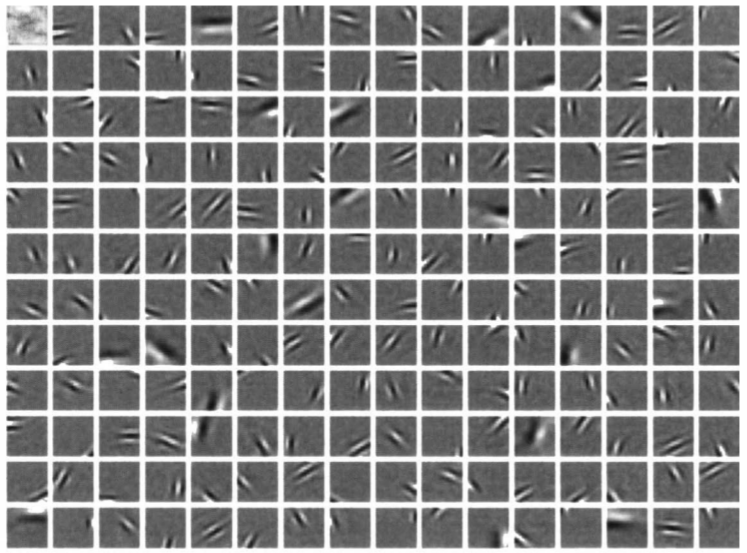
\includegraphics[width=12cm]{edges.png}
\end{center}
\caption{Sparse filters; the optimal features $W^s_{ij}$ using
  $16\times 16$ image patches cut from a corpus of pictures of the
  American northwest. [From \cite{OlshausenField1996a}].\label{fig:edges}}
\end{figure}

As described, none of this seems very biological, the sparse filters
were discovered using numerical optimization routines. However, there
are biologically plausible implementations using Hebbian learning, see
for example \cite{OReillyMunakata2000a}. There are other approach
which parallel sparseness as a way of distinguishing features, for
example, Infomax, which examines the informativeness of putative features \cite{BellSejnowski1995a}.


\begin{thebibliography}{10}

\bibitem{HubelWiesel1962a} Hubel DH, Wiesel TN. (1962) Receptive
  fields, binocular interaction and functional architecture in the
  cat's visual cortex.  \newblock The Journal of Physiology 160: 106.

\bibitem{OlshausenField1996a}
Olshausen BA, Field DJ (1996) Emergence of simple-cell receptive field properties by learning a sparse code for natural images. 
\newblock Nature, 381: 607--609.

\bibitem{OlshausenField1997a}
Olshausen BA, Field DJ (1997) Sparse coding with an overcomplete basis set: A strategy employed by V1?. 
\newblock Vision Research 37: 3311--3325.

\bibitem{OReillyMunakata2000a}
O'Reilly RC, Munakata Y (2000) Computational explorations in cognitive neuroscience: Understanding the mind by simulating the brain. 
\newblock MIT Press.

\bibitem{BellSejnowski1995a}
Bell AJ, Sejnowski TJ (1995) An information-maximization approach to blind separation and blind deconvolution. 
\newblock Neural Computation 7: 1129--1159.



\end{thebibliography}

\end{document}

